\chapter{Background}
\label{chapter2_background}
\thispagestyle{empty}

\vspace{0.5cm}

\noindent In this chapter we outline the theoretical framework which will be 
used in the following chapters. The approach proposed in this thesis draws 
equally from the fields of \textit{deep learning} and 
\textit{reinforcement learning}, in a hybrid setting usually called 
\textit{deep reinforcement learning}.

In the following sections we give high level descriptions of these
three fields, in order to introduce a theoretical background, a common notation, 
and a general view of some of the most important techniques in each area. 

\section{Deep Learning} \label{s:DL}
\textit{Deep Learning} (DL) is a branch of machine learning which aims to learn
abstract representations of the input space by means of complex function 
approximators.  Deep-learning methods are based on multiple levels of 
representation, obtained by composing simple but non-linear modules that each 
transform the representation at one level (starting with the raw input) into a 
representation at a higher, slightly more abstract level \cite{lecun2015deep}.

Deep learning has been at the heart of modern machine learning research, 
where deep models have revolutionized many fields like computer vision 
\cite{krizhevsky2012imagenet, szegedy2015going}, machine translation 
\cite{wu2016google} and speech synthesis \cite{vanwavenet}.
Generally, the most impressive results of deep learning have been achieved through
the versatility of \textit{neural networks}, which are universal function 
approximators well suited for hierarchical composition.

In this section we give a brief overview of the basic concepts behind 
\textit{deep neural networks }and introduce some important ideas that will be 
used in later chapters of this thesis.

\subsection{Artificial Neural Networks}
\textit{Feed-forward Artificial Neural Networks} (ANNs) \cite{bishop2006pattern} 
are universal function approximators inspired by the connected structure of 
neurons and synapses in biological brains.
%
\begin{figure}[H]
    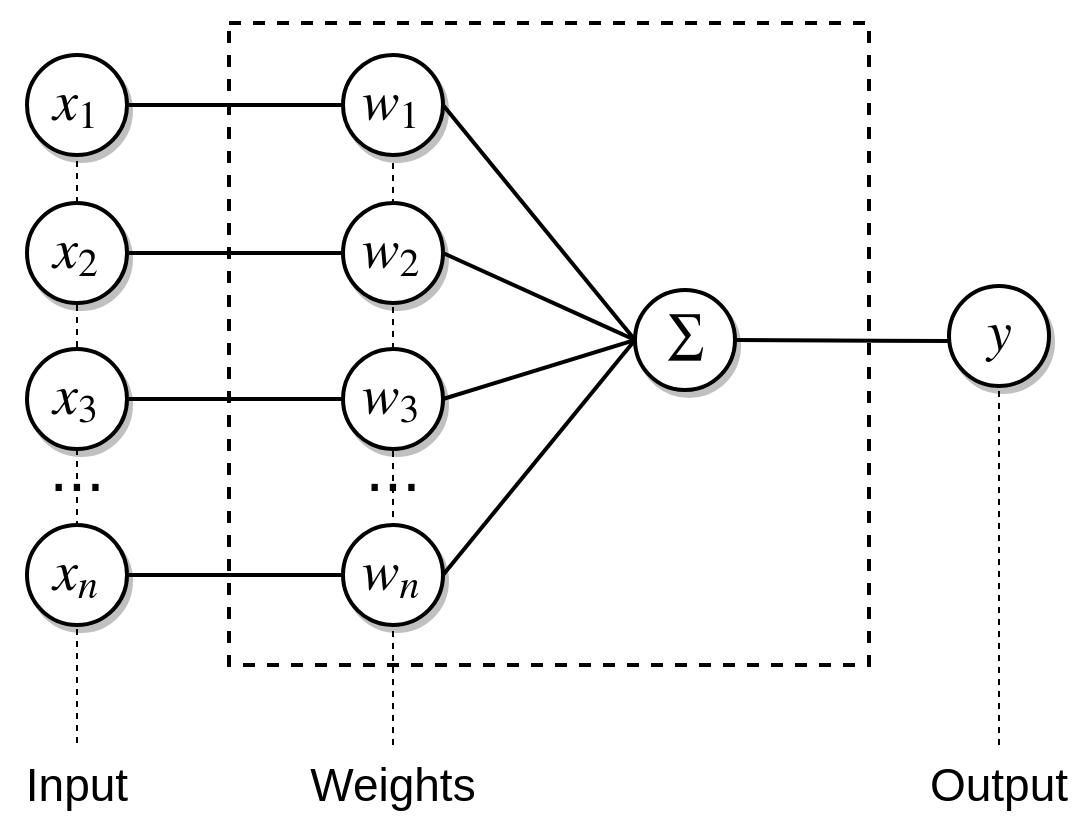
\includegraphics[width=0.6\textwidth]{pictures/perceptron}
    \centering
    \caption{graphical representation of the perceptron model.}
\end{figure}
%
ANNs are based on a fairly simple computational model called \textit{perceptron}, 
which is a transformation of an n-space into a scalar value
%
\begin{IEEEeqnarray}{rCl}
    %
    z = \sum\limits_{i = 1}^{n} (w_i \cdot x_i) + b
    %
\end{IEEEeqnarray}
%
where $x = (x_1, ..., x_n)$ is the $n$-dimensional input to the model, 
$w  = (w_1, ..., w_n)$ is a set of weights associated to each component of the 
input and $b$ is a bias term (in some notations the bias is embedded in the 
transformation by setting $x_0 = 1$ and $w_0 = b$).

In ANNs, the simple model of the perceptron is used to create a layered 
structure, in which each \textit{hidden} layer is composed by a given number 
of perceptrons (called \textit{neurons}) which:
%
\begin{enumerate}
    %
    \item take as input the output of the previous layer;
    \item are followed by a nonlinearity $\sigma$ called the \textit{activation
    function};
    \item output their value as a component of some $m$-dimensional space 
    which is the input space of the following layer.
    %
\end{enumerate}
%
\begin{figure}[h]
    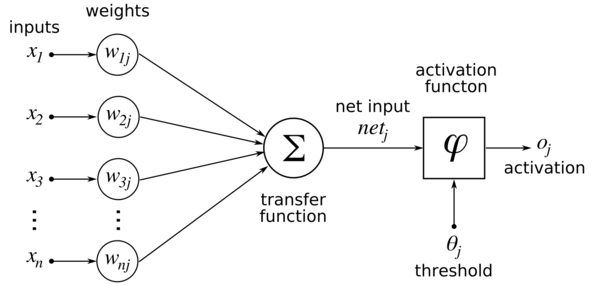
\includegraphics[width=0.6\textwidth]{pictures/neuron}
    \centering
    \caption{graphical representation of a neuron.}
\end{figure}
%
In simpler terms, each hidden layer computes an affine transformation of its 
input space:
%
    \begin{IEEEeqnarray}{rCl}
	%
	z^{(i)} = W^{(i)} \cdot \sigma(z^{(i-1)}) + B^{(i)}
	%
    \end{IEEEeqnarray}
%
where $W^{(i)}$ is the composition of the weights associated to each neuron in 
the layer and $B$ is the equivalent composition of the biases. 

The processing of the input space performed by the succession of layers which 
compose an ANN is equivalent to the composition of multiple non-linear 
transformations, which results in the production of an output vector on the 
co-domain of the target function.
%
\begin{figure}[h]
    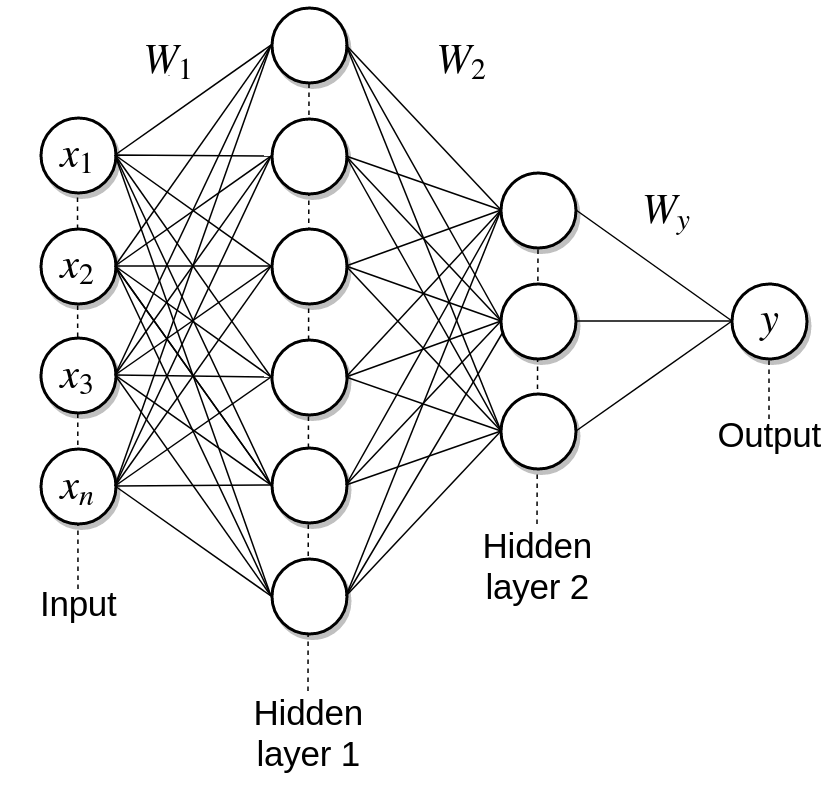
\includegraphics[width=0.6\textwidth]{pictures/ann}
    \centering
    \caption{a neural network with one hidden layer.}
\end{figure}
%

\subsection{Backpropagation}
Training ANNs is a parametric learning problem, where a \textit{loss} function 
is minimized starting from a collection of \textit{training samples} collected 
by the real process which is being approximated. In parametric learning the goal
is to find the optimal parameters of a mathematical model, such that the 
expected error made by the model on the training samples is minimized.
In ANNs, the parameters which are optimized are the weight matrices $W^{(i)}$ 
and biases $B^{(i)}$ associated to each hidden layer of the network. 

In the simple perceptron model, which basically computes a linear transformation
of the input, the optimal parameters are learned from the training set according
to the following \textit{update rule}:
%
\begin{IEEEeqnarray}{rCl}
    %
    w_i^{new} = w_i^{old} - \eta(\hat y -y) x_i, \forall i=(1, ..., n)
    %
\end{IEEEeqnarray}
%
where $\hat y$ is the output of the perceptron, $y$ is the real target from the
training set, $x_i$ is the $i$-th component of the input, and $\eta$ is a 
scaling factor called the \textit{learning rate} which regulates how much the 
weights are allowed to change in a single update. 
Successive applications of the update rule for the perceptron guarantee 
convergence to an optimum if and only if the approximated function is linear 
(in the case of regression) or the problem is linearly separable (in the case 
of classification).
%
\begin{figure}[h]
    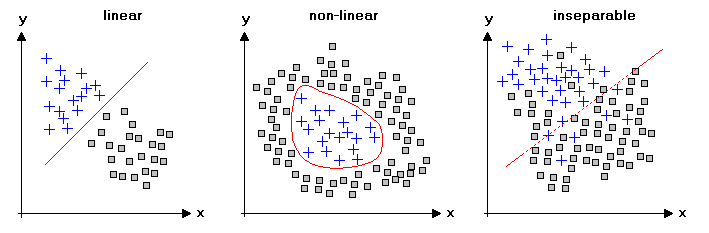
\includegraphics[width=\textwidth]{pictures/perceptron_separability}
    \centering
    \caption{different 2D classification problems, respectively linearly, 
	     non-linearly and non separable. The perceptron would be able to 
	     converge and correctly classify the points only in the first 
	     setting.}
\end{figure}
%

The simple update rule of the perceptron, however, cannot be used to train an ANN 
with multiple layers because the true outputs of the hidden layers are not
known a priori. 
To solve this issue, it is sufficient to notice that the function computed by 
each layer of a network is nonlinear, but differentiable with respect to the 
layer's input (i.e. it is linear in the weights).
This simple fact allows to compute the partial derivative of the loss function
for each weight matrix in the network to, in a sense, impute the error committed
on a training sample proportionally across neurons. The error is therefore 
propagated backwards (hence the name \textit{backpropagation}) to update all 
weights in a similar fashion to the perceptron update. 
The gradient of the loss function is then used to change the value of the 
weights, with a technique called \textit{gradient descent} which consists in 
the following update rule:
%
\begin{IEEEeqnarray}{rCl}
    %
    W_i^{new} = W_i^{old} - \eta \frac{\partial L(y, \hat y)}{\partial W_i^{old}}
    %
\end{IEEEeqnarray}
%
where $L$ is any differentiable function of the target and predicted values 
that quantifies the error made by the model on the training samples. The term 
\textit{gradient descent} is due to the fact that the weights are updated in
the opposite direction of the loss gradient, moving towards a set of parameters 
for which the loss is lower.
%
\begin{figure}[h]
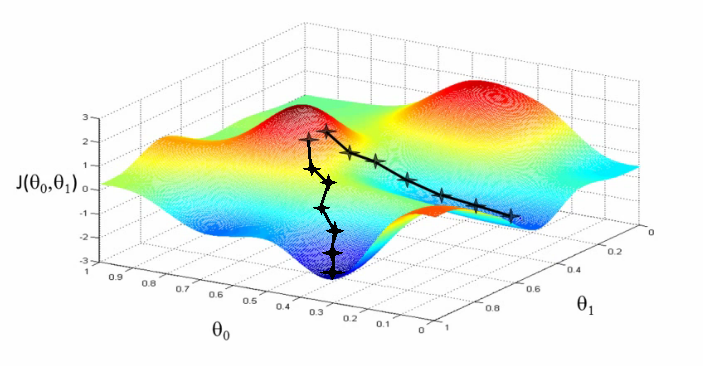
\includegraphics[width=0.8\textwidth]{pictures/SGD}
\centering
\caption{visualization of SGD on a space of two parameters.}
\end{figure}
%

Notice that traditional gradient descent optimizes the loss function over all 
the training set at once, performing a single update of the parameters. 
This approach, however, can be computationally expensive when the training set
is big; a more common approach is to use \textit{stochastic gradient descent} 
(SGD) \cite{bishop2006pattern}, which instead performs sequential parameters 
updates using small subsets of the training samples (called \textit{batches}). 
As the number of samples in a batch decreases, the variance of the 
updates increases, because the error committed by the model on a single sample 
can have more impact on the gradient step. This can cause the optimization algorithm 
to \textit{miss} a good local optima due to excessively big steps, but at the
same time could help leaving a poor local minima in which the optimization is
stuck. The same applies to the learning rate, which is the other important 
factor in controlling the size of the gradient step: if the learning rate is 
too big, SGD can \textit{overshoot} local minima and fail to converge, but at
the same time it may take longer to find the optimum if the learning rate is 
too small.
%
\begin{figure}[h]
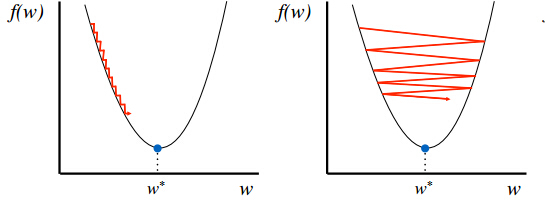
\includegraphics[width=0.6\textwidth]{pictures/SGD_overshooting}
\centering
\caption{effect of the learning rate on SGD updates. Too small (left) may 
	 take longer to converge, too big (right) may \textit{overshoot} the
	 optimum and even diverge.}
\end{figure}
%

In order to improve the accuracy and speed of SGD, some additional tweaks are
usually added to the optimization algorithm. Among these, we find the addition
of a \textit{momentum} term to the update step of SGD, in order to avoid 
oscillating in irrelevant directions by incorporating a fraction of the previous
update term in the current one:
%
\begin{IEEEeqnarray}{rCl}
    %
    W_i^{(j+1)} = W_i^{(j)} - \gamma \eta \frac{\partial L(y^{(j-1)}, \hat y^{(j-1)})}{\partial W_i^{(j-1)}} - \eta \frac{\partial L(y^{(j)}, \hat y^{(j)})}{\partial W_i^{(j)}}
    %
\end{IEEEeqnarray}
%
where $(j)$ is the number of updates that have occurred so far. In this approach, 
momentum has the same meaning as in physics, like when a body falling
down a slope tends to preserve part of its previous velocity when subjected
to a force. 
Other techniques to improve convergence include the use of an adaptive 
learning rate based on the previous gradients computed for the weights (namely
the \textit{Adagrad} \cite{duchi2011adaptive} and \textit{Adadelta} 
\cite{zeiler2012adadelta} optimization algorithms), and a similar approach 
which uses an adaptive momentum term (called \textit{Adam} \cite{kingma2014adam}).

\subsection{Convolutional Neural Networks} \label{s:CNN}
\textit{Convolutional Neural Networks} (CNNs) are a type of ANN inspired by the 
visual cortex in animal brains, and have been widely used in recent literature 
to reach state-of-the-art results in fields like computer vision, machine 
translation, and, as we will see in later sections, reinforcement learning.

CNNs exploit spatially-local correlations in the neurons of adjacent 
layers by using a \textit{receptive field}, a set of weights which is used to 
transform a local subset of the input neurons of a layer.
The receptive field is applied as a \textit{filter} over different locations of 
the input, in a fashion that resembles how a signal is \textit{strided} across 
the other during convolution. 
The result of this operation is a nonlinear transformation of 
the input space into a new space (of compatible dimensions) which preserves
the spatial information encoded in the input (e.g. form the $n \times m$ pixels
of a grayscale image to a $j \times k$ matrix that represents subgroups of 
pixels in which there is an edge).
%
\begin{figure}[h]
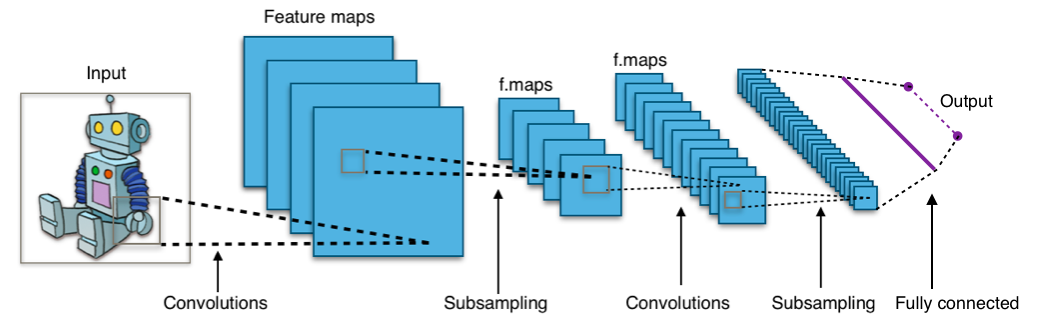
\includegraphics[width=	\textwidth]{pictures/CNN}
\centering
\caption{typical structure of a deep convolutional neural network for image
	 processing, with two convolutional hidden layers and a dense section
	 at the end (for classification or regression).}
\end{figure}
%

While standard ANNs have a \textit{fully connected} (sometimes also called 
\textit{dense}) structure, with each neuron of a layer connected to each neuron 
of the previous and following layer, in CNNs the weights are associated to a 
filter and \textit{shared} across all neurons of a layer. 
This \textit{weights sharing} has the double advantage of greatly reducing the 
number of parameters that must be updated during training, and of forcing the 
network to learn general abstractions of the input that can be applied to any 
subset of neurons covered by the filter.
%
\begin{figure}[h]
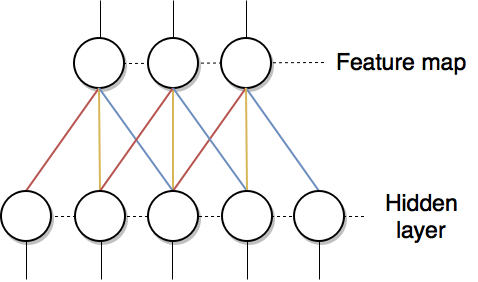
\includegraphics[width=0.5\textwidth]{pictures/shared_weights}
\centering
\caption{simple representation of shared weights in a 1D CNN. Each neuron in 
	 the second layer applies the same receptive field of three weights
	 to three adjacent neurons of the previous layer. The filter is applied 
	 with a stride of one element to produce the feature map.}
\end{figure}
%

In general, the application of a filter is not limited to one per layer and it 
is customary to have more than one filter applied to the same input in parallel,
to create a set of independent abstractions called \textit{feature maps} (also
referred to as \textit{channels}, to recall the terminology of RGB images for 
which a 3-channel representation is used for red, green, and blue). In 
this case, there will be a set of shared weights for each filter.
When a set of feature maps is given as input to a convolutional layer, a 
multidimensional filter is strided simultaneously across all channels.

At the same time, while it may be useful to have parallel abstractions of the 
input space (which effectively enlarges the output space of the layers), it is
also necessary to force a reduction of the input in order to learn useful 
representations. 
For this reason, convolutional layers in CNNs are often paired with 
\textit{pooling layers} which reduce the dimensionality of their input according
to some criteria applied to subregions of the input neurons (e.g. for each two 
by two square of input neurons, keep only the maximum activation value).
%
\begin{figure}[h]
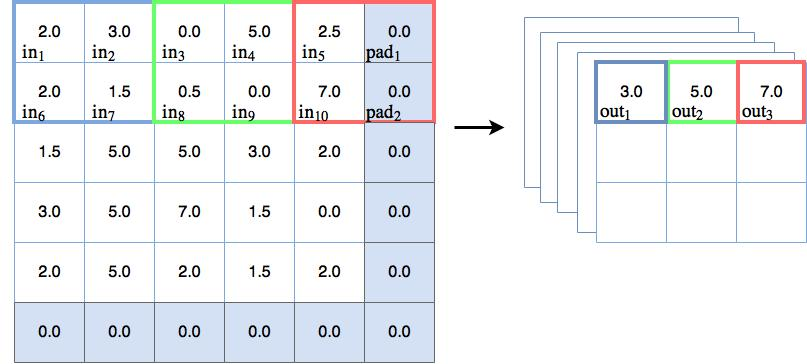
\includegraphics[width=0.7\textwidth]{pictures/max-pooling}
\centering
\caption{example of \textit{max pooling}, where only the highest activation 
	 value in the pooling window is kept.}
\end{figure}
%

Finally, typical applications of CNNs in the literature use mixed 
architectures composed of both convolutional and fully connected layers.
In tasks like image classification \cite{simonyan2014vggnet, szegedy2015going}, 
convolutional layers are used to extract significant features directly from the 
images, and dense layers are used as a final classification model; the training 
in this case is done in an end-to-end fashion, with the classification error 
being propagated across all layers to \textit{fine-tune} all weights and filters
to the specific problem.

\subsection{Autoencoders}
Autoencoders (AE) are a type of ANN which is used to learn a sparse and 
compressed representation of the input space, by sequentially compressing and 
reconstructing the inputs under some sparsity constraint.

The typical structure of an AE is split into two sections: an 
\textit{encoder} and a \textit{decoder}. In the classic architecture of 
autoencoders these two components are exact mirrors of one another, but in 
general the only constraint that is needed to define an AE is that
the dimensionality of the input be the same as the dimensionality of the output.
In general, however, the last layer of the encoder should output a reduced 
representation of the input which contains enough information for the decoder to
invert the transformation.
%
\begin{figure}[h]
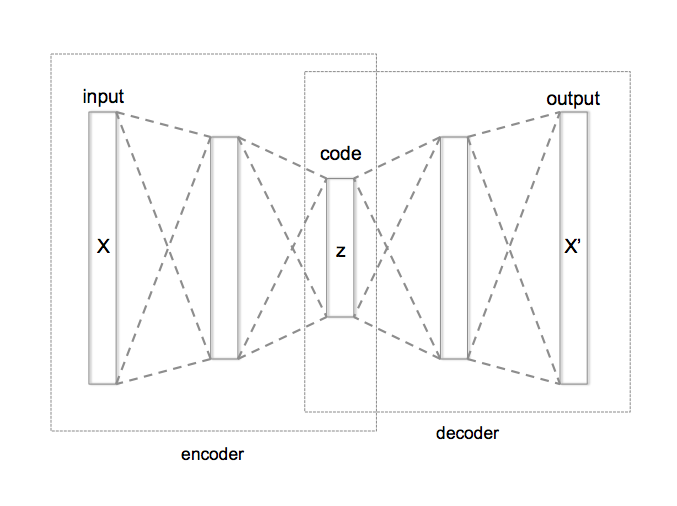
\includegraphics[width=0.7\textwidth]{pictures/autoencoder}
\centering
\caption{schematic view of an autoencoder, with the two main components 
	 highlighted.}
\end{figure}
%

The training of an AE is done in an unsupervised fashion, with no
explicit target required as the network is simply trained to predict its input.
Moreover, a strong regularization constraint is often imposed on the innermost 
layer to ensure that the learned representation is as abstract as possible 
(typically the $L1$ norm of the activations is minimized as additional term to
 the loss, to enforce sparsity). 

Autoencoders can be especially effective in extracting meaningful
features from the input space, without tailoring the features to a specific 
problem like in the end-to-end image classification example of Section 
\ref{s:CNN} \cite{erhan2010does}. 
An example of this is the extraction of features from images, 
where convolutional layers are used in the encoder to obtain an abstract 
description of the image's structure. In this case, the decoder uses
convolutional layers to transform subregions of the representation, but the 
expansion of the compressed feature space is delegated to \textit{upscaling 
layers} (the opposite of pooling layers) \cite{masci2011cae}.
This approach in building the decoder, however, can sometimes cause blurry
or inaccurate reconstructions due to the upscaling operation which simply 
replicates information rather than transforming it (like pooling layers do).
Because of this, a more sophisticated technique has been developed recently 
which allows to build purely convolutional autoencoders, without the need of 
upscaling layers in the decoder.
The layers used in this approach are called \textit{deconvolutional}\footnote{Or
\textit{transposed convolutions}.} and are thoroughly presented in 
\cite{zeiler2010deconvolutional}. For the purpose of this thesis it suffices to 
notice that image reconstruction with this type of layer is incredibly more 
accurate, down to pixel-level accuracy.

\section{Reinforcement Learning} \label{s:RL}
\textit{Reinforcement Learning} (RL) is an area of machine learning which
studies how to optimize the behavior of an agent in an environment,
in order to maximize the cumulative sum of a scalar signal called 
\textit{reward} in a setting of \textit{sequential decision making}.
RL has its roots in optimization and control theory but, because of the generality 
of its characteristic techniques, it has been applied to a variety of scientific 
fields where the concept of \textit{optimal behavior in an environment} can be 
applied (examples include game theory, multi-agent systems and economy).
The core aspect of reinforcement learning problems is to represent the setting
of an agent performing decisions in an environment, which is in turn affected by
the decisions; a scalar reward signal represents a time-discrete indicator of 
the agent's performance. This kind of setting is inspired to the natural 
behavior of animals in their habitat, and the techniques used in reinforcement 
learning are well suitable to describe, at least partially, the complexity of
living beings. 

In this section we introduce the basic setting of RL and go over a brief 
selection of the main techniques used to solve RL problems. 
%
\begin{figure}[h]
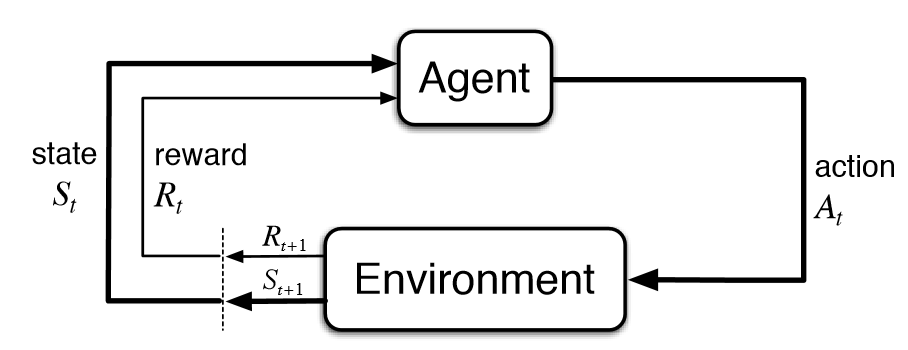
\includegraphics[width=0.7\textwidth]{pictures/reinforcement}
\centering
\caption{the reinforcement learning setting, with the agent performing actions
	 on the environment and in turn observing the state and reward.}
\end{figure}
%

\subsection{Markov Decision Processes}
\textit{Markov Decision Processes} (MDPs) are discrete-time, stochastic control 
processes, that can be used to describe the interaction of an \textit{agent} 
with an \textit{environment}.

Formally, MDPs are defined as 7-tuples $<S, S^{T}, A, P, R, \gamma, \mu>$, 
where:
\begin{itemize}
    %
    \item $S$ is the set of observable states of the environment.
    When the set if observable states coincides with the true set of states of the 
    environment, the MDP is said to be \textit{fully observable}. We will only 
    deal with fully observable MDPs without considering the case of 
    \textit{partially observable} MDPs.

    \item $S^{T} \subseteq S$ is the set of \textit{terminal states} of the 
    environment, meaning those states in which the interaction between the agent
    and the environment ends. The sequence of events that occur from when the
    agent observes an initial state until it reaches a terminal state is 
    usually called \textit{episode}.
 
    \item $A$ is the set of actions that the agent can execute in the 
    environment.
 
    \item $P: S \times A \times S \rightarrow [0,1]$ is a \textit{state 
    transition function} which, given two states $s, s' \in S$ and an action 
    $a \in A$, represents the probability of the agent going to state $s'$ by 
    executing $a$ in $s$.
 
    \item $R: S \times A \rightarrow \mathbb{R}$ is a \textit{reward function} 
    which represents the reward that the agent collects by executing an action 
    in a state. 
    
    \item $\gamma \in [0,1]$ is a \textit{discount factor} which is used to 
    weight the importance of rewards during time: $\gamma = 0$ means that only
    the immediate reward is considered, $\gamma = 1$ means that all rewards have
    the same importance.
    
    \item $\mu: S \rightarrow [0, 1]$ is a probability distribution over $S$ 
    which models the probability of starting the exploration of the environment 
    in a given state.
    %
\end{itemize}
%
\begin{figure}[h]
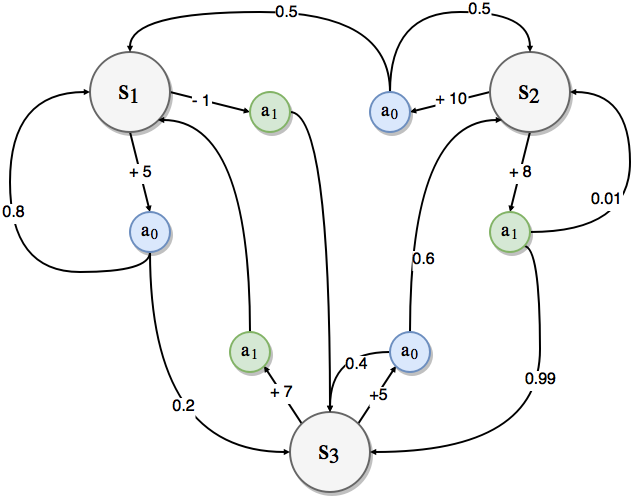
\includegraphics[width=0.5\textwidth]{pictures/mdp}
\centering
\caption{graph representation of an MDP. Each node represents a state, each arc
	 is a transition from a state to another; note that actions may have 
	 probability distributions associated to the following states.}
\end{figure}
%

Episodes are usually represented as sequences of tuples 
\[
    [(s_0, a_0, r_1, s_1), ..., (s_{n-1}, a_{n-1}, r_n, s_n)]
\]
called \textit{trajectories}, where $s_n \in S^T$, and $(s_i, a_i, r_{i+1}, s_{i+1})$ 
represents a transition of the agent to state $s_{i+1}$ by taking action $a_i$ 
in $s_i$ and collecting a reward $r_{i+1}$.

In MDPs the modeled environment must satisfy the \textit{Markov property}, 
meaning that the reward and transition functions of the environment must only 
depend on the current state and action, and not on the past state-action 
trajectory of the agent.
In other words, an environment is said to satisfy the Markov property when its 
one-step dynamics allow to predict the next state and reward given only the 
current state and action.

\subsubsection{Policy}
The behavior of the agent in an MDP can be defined as a probability 
distribution $\pi: S \times A \rightarrow [0,1]$ called a \textit{policy}, 
which given $s \in S, a \in A$, represents the probability of selecting $a$ as 
next action from $s$.
An agent which uses this probability distribution to select its next action 
when in a given state is said to be \textit{following} the policy.

A common problem when defining policies is the \textit{exploration-exploitation}
dilemma. An agent following a policy may end up observing the same trajectories 
in all episodes (e.g., when following a deterministic policy in a deterministic 
MDP), but there may be cases in which a better behavior could be had if the agent
\textit{explored} other states instead of simply \textit{exploiting} its 
knowledge. 
It is therefore common to add a probabilistic element to policies (irrespectively
of their determinism, a priori), in order to explicitly control the exploration
degree of the agent. Common techniques to control the 
\textit{exploration-exploitation} tradeoff are:
%
\begin{itemize}
    \item $\varepsilon$-greedy policies: actions are selected using a given 
    policy with probability $1-\varepsilon$, and randomly the rest of the time;
    \item softmax action selection: improves on $\varepsilon$-greedy policies by 
    reducing the number of times a suboptimal action is randomly selected. To do
    so, a probability distribution (commonly a \textit{Boltzmann distribution}) 
    dependent on the expected return from the successor states (something called
    the \textit{value} of the states, which is introduced in the next Subsection)
    is used.
\end{itemize}
%
\subsubsection{Value Functions}
Starting from the concept of policy, we can now introduce a function that 
evaluates how good it is for an agent following a policy $\pi$ to be in a given 
state. This evaluation is expressed in terms of the expected return, i.e.
the expected discounted sum of future rewards collected by an agent starting 
from a state while following $\pi$, and the function that computes it is 
called the \textit{state-value function for policy $\pi$} (or, more commonly, 
just \textit{value function}).

Formally, the state-value function associated to a policy $\pi$ is a function 
$V^{\pi}: S \rightarrow \mathbb{R}$ defined as:
%
\begin{IEEEeqnarray}{rCl}
    % Sutton, Barto
    V^{\pi}(s) & = & E_\pi[R_t | s_t = s] \\
    & = & E_\pi[\sum\limits_{k = 0}^{\infty} \gamma^k r_{t+k+1} | s_t = s]
    %
\end{IEEEeqnarray}
%
where $E_\pi[\cdot]$ is the expected value given that the agent follows 
policy $\pi$, and $t$ is any time step of an episode $[s_0, ..., s_t, ..., s_n]$
where $s_t \in S, \forall t = 0, ..., n$.

Similarly, we can also introduce a function that evaluates the goodness of 
taking a specific action in a given state, namely the expected reward obtained 
by taking an action $a \in A$ in a state $s \in S$ and then following policy 
$\pi$. 
We call this function the \textit{action-value function for policy $\pi$} 
denoted $Q^{\pi}: S \times A \rightarrow \mathbb{R}$, and defined as: 
%
\begin{IEEEeqnarray}{rCl}
    % Sutton, Barto
    Q^{\pi}(s, a) & = & E_\pi[R_t | s_t = s, a_t = a] \\
    & = & E_\pi[\sum\limits_{k = 0}^{\infty} \gamma^k r_{t+k+1} | s_t = s, a_t = a]
    %
\end{IEEEeqnarray}
%
The majority of reinforcement learning algorithms is based on computing (or 
estimating) value functions, which can then be used to control the behavior 
of the agent.
We also note a fundamental property of value functions, which satisfy particular 
recursive relationships like the following \textit{Bellman equation for 
$V^{\pi}$}:
%
\begin{IEEEeqnarray}{rCl}
    % Sutton, Barto
    V^{\pi}(s) & = & E_\pi[R_t | s_t = s] \nonumber\\
    & = & E_\pi[\sum\limits_{k = 0}^{\infty} \gamma^k r_{t+k+1} | s_t = s] \nonumber\\
    & = & E_\pi[r_{t+1} + \gamma \sum\limits_{k=0}^{\infty} \gamma^k r_{t+k+2} | s_t = s] \\
    & = & \sum\limits_{a \in A} \pi(s, a) \sum\limits_{s' \in S} P(s, a, s')[R(s, a) \>+ \nonumber\\
    && +\> \gamma E_\pi[\sum\limits_{k=0}^{\infty} \gamma^k r_{t+k+2} | s_{t+1} = s']] \\
    & = & \sum\limits_{a \in A} \pi(s, a) \sum\limits_{s' \in S} P(s, a, s')[R(s, a) + \gamma V^{\pi}(s')] \label{eq:BEV}
    %
\end{IEEEeqnarray}
%
Intuitively, relation \eqref{eq:BEV} decomposes the state-value function as the 
sum of the immediate reward collected from a state $s$ to a successor state 
$s'$, and the value of $s'$ itself; by considering the transition model of the 
MDP and the policy being followed, we see that the Bellman equation simply 
averages the expected return over all the possible $(s, a, r, s')$ transitions, 
by taking into account the probability that these transitions occur. 

\subsection{Optimal Value Functions}
In general terms, \textit{solving} a reinforcement learning task consists in 
finding a policy that yields a sufficiently high expected return. In the case of
MDPs with finite state and actions sets\footnote{We make this clarification for 
formality, but we do not expand the details further in this work. Refer to 
\cite{sutton1998reinforcement} for more details on the subjet of non-finite MDPs.}, 
it is possible to define the concept of \textit{optimal policy} as the policy 
which maximizes the expected return collected by the agent in an episode.

We start by noticing that state-value functions define a partial ordering over 
policies as follows: 
\[
    \pi \ge \pi' \iff V^{\pi}(s) \ge V^{\pi'}(s), \forall s \in S
\]
From this, the \textit{optimal policy $\pi^*$} of an MDP is a policy which is
better or equal than all other policies in the policy space. It has also been 
proven that among all optimal policies for an MDP, there is always a 
deterministic one (see Section \ref{s:value_based_optimization}).

The state-value function associated to $\pi^*$ is called the 
\textit{optimal state-value function}, denoted $V^*$ and defined as:
%
\begin{IEEEeqnarray}{rCl}
    % Sutton, Barto
    V^*(s) = \max_{\pi} V^\pi(s), \forall s \in S
    %
\end{IEEEeqnarray}
%
As we did when introducing the value functions, given an optimal policy for the 
MDP it is also possible to define the \textit{optimal action-value function} 
denoted $Q^*$:
%
\begin{IEEEeqnarray}{rCl}
    % Sutton, Barto
    Q^*(s, a) & = & \max_{\pi} Q^\pi(s, a) \\
    & = & E[r_{t+1} + \gamma V^*(s_{t+1}) | s_t = s, a_t = a] \label{eq:Qstar_V}
    %
\end{IEEEeqnarray}
%
Notice that equivalence \eqref{eq:Qstar_V} in this definition highlights the 
relation between $Q^*$ and $V^*$.

Since $V^*$ and $Q^*$ are value functions of an MDP, they must satisfy the same
type of recursive relations that we described in \eqref{eq:BEV}, in this case
called the \textit{Bellman optimality equations}.
The Bellman optimality equation for $V^*$ expresses the fact that the value of
a state associated to an optimal policy must be the expected return of the best
action that the agent can take in that state:
%
\begin{IEEEeqnarray}{rCl}
    % Sutton, Barto
    V^*(s) & = & \max_a Q^*(s, a) \label{eq:BOEV}\\
    & = & \max_a E_{\pi^*}[R_t | s_t = s, a_t = a] \\
    & = & \max_a E_{\pi^*}[\sum\limits_{k=0}^{\infty} \gamma^k r_{t+k+1}| s_t = s, a_t = a] \\
    & = & \max_a E_{\pi^*}[r_{t+1} + \gamma \sum\limits_{k=0}^{\infty} \gamma^k r_t+k+2 | s_t = s, a_t = a] \\
    & = & \max_a E_{\pi^*}[r_{t+1} + \gamma V^*(s_{t+1}) | s_t = s, a_t = a] \\
    & = & \max_a \sum\limits_{s' \in S} P(s, a, s') [ R(s, a) + \gamma V^*(s') ]
    %
\end{IEEEeqnarray}
%
The Bellman optimality equation for $Q^*$ is again obtained from the definition
as:
%
\begin{IEEEeqnarray}{rCl}
    % Sutton, Barto
    Q^*(s, a) & = & E[ r_{t+1} + \gamma \max_{a'} Q^*(s_{t+1}, a') | |s_t = s, a_t = a] \\
    & = & \sum\limits_{s'} P(s, a, s') [ R(s, a) + \gamma \max_{a'}Q^*(s', a') ]
    %
\end{IEEEeqnarray}
%
Notice that both Bellman optimality equations have a unique solution independent 
of the policy. 
If the dynamics of the environment ($R$ and $P$) are fully known, it is possible
to solve the system of equations associated to the value functions (i.e. one
equation for each state in $S$) and get an exact value for $V^*$ and $Q^*$ in 
each state. 

\subsection{Value-based optimization} \label{s:value_based_optimization}
One of main algorithm classes for solving reinforcement learning problems
is based on searching an optimal policy for the MDP by computing either 
of the optimal value functions, and then deriving a policy based on them.
From $V^*$ or $Q^*$, it is easy to determine an optimal, deterministic policy:
\begin{itemize}
    %
    \item Given $V^*$, for each state $s \in S$ there will be an action (or 
    actions) which maximizes the Bellman optimality equation \eqref{eq:BOEV}. 
    Any policy that assigns positive probability to only this action is an 
    optimal policy.
    This approach therefore consists in performing a one-step forward search on 
    the state space to determine the best action from the current state.
    \item Given $Q^*$, the optimal policy is that which assigns positive 
    probability to the action which maximizes $Q^*(s, a)$; this approach 
    exploits the intrinsic property of the action-value function of representing 
    the \textit{quality} of actions, without performing the one-step search 
    on the successor states. 
    %
\end{itemize}

In the following sections we will describe some of the most important value-based 
approaches to RL, which will be useful in the following chapters of this thesis. 
We will not deal with equally popular methods like \textit{policy gradient} or 
\textit{actor-critic} approaches, even though they have been successfully 
applied in conjunction with DL to solve complex environments (see Section 
\ref{s:DRL} and Chapter \ref{chapter3_state_of_the_art}).

\subsection{Dynamic Programming}
The use of dynamic programming (DP) techniques to solve reinforcement learning 
problems is based on recursively applying some form of the Bellman equation, 
starting from an initial policy $\pi$ until convergence to $\pi^*$.
In this class of algorithms, we identify two main approaches: \textit{policy 
iteration} and \textit{value iteration}.

\subsubsection{Policy iteration}
%
\begin{figure}[h]
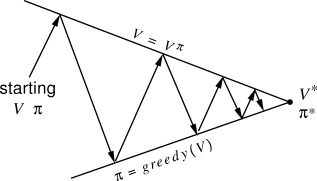
\includegraphics[width=0.5\textwidth]{pictures/policyiter}
\centering
\caption{classical representation of the policy iteration algorithm, which
	 highlights the relation between policies and their associated value
	 functions. Each pair of arrows starting from a policy and ending on a
	 greedy policy based on the value function is a step of the algorithm.}
\end{figure}
%
\textit{Policy iteration} is based of the following theorem:
\begin{theorem}[Policy improvement theorem] \label{th:pol_imp}
    % Lecture 11, slide 18
    Let $\pi$ and $\pi'$ be a pair of deterministic policies such that
    \[
        Q^\pi(s, \pi'(s)) \ge V^\pi(s), \forall s \in S 
    \]
    Then, $\pi' \ge \pi$, i.e. 
    \[
        V^{\pi'}(s) \ge V^{\pi}(s), \forall s \in S
    \]
    %
\end{theorem}

This approach works by iteratively computing the value function associated to 
the current policy, and then improving that policy by making it act greedily 
with respect to the value function, such that:
%
\begin{IEEEeqnarray}{rCl}
    % Lecture 11, slide 17
    \pi'(s) = \underset{a \in A}{\arg\max} Q^{\pi}(s, a) \label{eq:greedy_imp}
    %
\end{IEEEeqnarray}
%
For Theorem \ref{th:pol_imp}, the expected return of the policy is thus improved
because:
%
\begin{IEEEeqnarray}{rCl}	
    % Lecture 11, slide 17
    Q^\pi(s, \pi'(s)) = \max_{a \in A} Q^\pi(s, a) \ge Q^\pi(s, \pi(s)) = V^\pi(s) \label{eq:policy_improv}
\end{IEEEeqnarray}
%
This continuous improvement is applied until the inequality in \eqref{eq:policy_improv} 
becomes an equality, i.e. until the improved policy satisfies the 
Bellman optimality equation \eqref{eq:BOEV}. Since the algorithm gives no 
assurances on the number of updates required for convergence, some stopping
conditions are usually introduced to end the process when the new value function 
does not change substantially after the update (\textit{$\varepsilon$-convergence}) 
or a certain threshold number of iterations has been reached.

\subsubsection{Value iteration} \label{s:value_iteration}
Starting from a similar idea, the \textit{value iteration} approach computes 
the value function associated to an initial policy, but then applies a 
contraction operator which iterates over sequentially better value functions 
without actually computing the associated greedy policy.
The contraction operator which ensures convergence is the \textit{Bellman 
optimality backup}:
%
\begin{IEEEeqnarray}{rCl}
    % Sutton, Barto (p.266)
    V_{k+1}(s) \leftarrow \max_a \sum\limits_{s'}P(s, a, s')[R(s, a) + \gamma V(s')]
    %
\end{IEEEeqnarray}
%
As with policy iteration, convergence is ensured without guarantees on 
the number of steps, and therefore it usual to terminate the iteration according
to some stopping condition.

\subsection{Monte Carlo Methods}
Dynamic programming approaches exploit the exact solution of a value function 
which can be computed starting from a policy, but in general this requires to 
have a perfect knowledge of the environment's dynamics and may also not be 
tractable on sufficiently complex MDPs. 

\textit{Monte Carlo} (MC) methods are a way of solving reinforcement learning 
problems by only using \textit{experience}, i.e. a collection of \textit{sample 
trajectories} from an actual interaction of an agent with the environment.
This is often referred to as a \textit{model-free} approach because, while the
environment (or a simulation thereof) is still required to observe the sample
trajectories, it is not necessary to have an exact knowledge of the transition 
model and reward function of the MDP. 

Despite the differences with dynamic programming, this approach is still 
based on the same two-step process of policy iteration (evaluation and 
improvement).
To estimate the value of a state $V^\pi(s)$ under a policy $\pi$ with Monte 
Carlo methods, it is sufficient to consider a set of episodes collected under 
$\pi$: the value of the state $s$ will be computed as the average of the returns 
collected following a \textit{visit} of the agent to $s$, for all occurrences of
$s$ in the collection\footnote{Note that a variation of this 
algorithm exists, which only considers the average returns following the 
\textit{first} visit to a state in each episode.}.

This same approach can be also used to estimate the action-value function, 
simply by considering the occurrence of state-action pairs in the collected 
experience rather than states only. 

Finally, the policy is improved by computing its greedy variation \eqref{eq:greedy_imp}
with respect to the estimated value functions and the process is iteratively
repeated until convergence, with a new set of trajectories collected under each 
new policy.

\subsection{Temporal Difference Learning}
\textit{Temporal Difference} (TD) learning is an approach to RL which uses 
concepts from both dynamic programming and Monte Carlo techniques. 
TD is a \textit{model-free} approach which uses experience (like in MC)
to update an estimate of the value functions by using a previous estimate 
(like in DP).
Like MC, TD estimation uses the rewards following a visit to a state to compute
the value functions, but with two core differences:
\begin{enumerate}
    %
    \item Instead of the average of all rewards following the visit, a single 
    time step is considered (this is true for the simplest TD approach, but note 
    that in general an arbitrary number of steps can be used; the more steps are
    considered, the more the estimate is similar to the MC estimate).
    \item Estimates of the value functions are updated by using in part an 
    already computed estimate. For this reason, this approach is called a
    \textit{bootstrapping} method (like DP).
    Specifically, the iterative update step for the value function is:
    %
    \begin{IEEEeqnarray}{rCl}
	%
	V(s_t) \leftarrow V(s_t) + \alpha[r_{t+1} + \gamma V(s_{t+1}) - V(s_t)]
	%
    \end{IEEEeqnarray}
    %
    %
\end{enumerate}

In general, TD methods have several advantages over MC as they allow for an 
\textit{on-line} (i.e. they don't require full episode trajectories to work), 
bootstrapped, \textit{model-free} estimate, which is more suitable for problems 
with long or even infinite time horizons. Moreover, TD is less susceptible to 
errors or exploratory actions and in general provides a more stable learning.
It must be noted, however, that both TD and MC are guaranteed to converge given 
a sufficiently large amount of experience, and that there are problems for which 
either of the two can converge faster to the solution.

We will now present the two principal control algorithms in the TD family, one 
said to be \textit{on-policy} (i.e. methods that attempt to evaluate and improve 
the same policy that they use to make decisions) and the other 
\textit{off-policy} (i.e. methods with no relations between the estimated policy
and the policy used to collect experience).

\subsubsection{SARSA}
As usual in \textit{on-policy} approaches, \textit{SARSA}\footnote{Originally 
called \textit{on-line Q-learning} by the creators; this alternative acronym was 
proposed by Richard Sutton and reported in a footnote of the original paper in 
reference to the \textit{State, Action, Reward, next State, next Action} tuples 
which are used for prediction.} works by estimating the value $Q^\pi(s, a)$ for 
a current behavior policy $\pi$ which is used to collect sample transitions from
the environment.
The policy is updated towards greediness with respect to the estimated 
action-value after each transition $(s, a, r, s', a')$, and the action-value
is in turn updated step-wise with the following rule: 
%
\begin{IEEEeqnarray}{rCl}
    %
    Q(s_t, a_t) \leftarrow Q(s_t, a_t) + \alpha [r_{t+1} + \gamma Q(s_{t+1}, a_{t+1}) - Q(s_t,  a_t)] \label{eq:SARSA_update}
    %
\end{IEEEeqnarray}
%
The training procedure of SARSA can be summarized with Algorithm \ref{alg:SARSA}.
%
\begin{algorithm}[h]
    \caption{SARSA}
    \label{alg:SARSA}
    \begin{algorithmic}
        \STATE Initialize $Q(s,a)$ arbitrarily
        \STATE Initialize $\pi$ as some function of $Q$ (e.g. greedy)
        \REPEAT
	    \STATE Initialize $s$
	    \STATE Choose $a$ from $s$ using $\pi$
	    \REPEAT	
		\STATE Take action $a$, observe $r$, $s'$
		\STATE Choose $a'$ from $s'$ using $\pi$
		\STATE Update $Q(s, a)$ using rule \eqref{eq:SARSA_update}
		\IF{$\pi$ is time-variant}
		    \STATE Update $\pi$ towards greediness
		\ENDIF
		\STATE $s \leftarrow s'$; $a \leftarrow a'$
	    \UNTIL{$s$ is terminal or Q did not change}
	\UNTIL{training ended or Q did not change}
    \end{algorithmic}
\end{algorithm}
%

Convergence of the SARSA method is guaranteed by the dependence of $\pi$ on the
action-value function, as long as all state-action pairs are visited an infinite
number of times and the policy converges in the limit to the greedy policy (e.g. 
a time-dependent $\varepsilon$-greedy policy with $\varepsilon = 1/t$).

\subsubsection{Q-learning}
Defined by Sutton and Barto \cite{sutton1998reinforcement} as one of the most 
important breakthroughs in reinforcement learning, \textit{Q-learning} is an 
\textit{off-policy} temporal difference method that approximates the optimal 
action-value function independently of the policy being used to collect 
experiences. 
This simple, yet powerful idea guarantees convergence to the optimal 
value function as long as all state-action pairs are continuously visited (i.e. 
updated) during training.

The update rule for the TD step in Q-learning is the following: 
%
\begin{IEEEeqnarray}{rCl}
    %
    Q(s_t, a_t) \leftarrow Q(s_t, a_t) + \alpha [r_{t+1} + \gamma \max_a Q(s_{t+1}, a) - Q(s_t,  a_t)] \label{eq:QL_update}
    %
\end{IEEEeqnarray}
%
As we did for SARSA, an algorithmic description of the Q-learning algorithm is
provided in Algorithm \ref{alq:q_learning}.
%
\begin{algorithm}[h]
    \caption{Q-Learning}
    \label{alq:q_learning}
    \begin{algorithmic}
        \STATE Initialize $Q(s,a)$ and $\pi$ arbitrarily
        \REPEAT
	    \STATE Initialize $s$
	    \REPEAT	
		\STATE Choose $a$ from $s'$ using $\pi$
		\STATE Take action $a$, observe $r$, $s'$
		\STATE Update $Q(s, a)$ using rule \eqref{eq:QL_update}
		\STATE $s \leftarrow s'$
	    \UNTIL{$s$ is terminal or Q did not change}
	\UNTIL{training ended or Q did not change}
    \end{algorithmic}
\end{algorithm}
%

\subsection{Fitted Q-Iteration}
Having introduced a more classic set of traditional RL algorithms in the 
previous sections, we now present a more modern approach to solve MDPs with the 
use of supervised learning algorithms to estimate the value functions.

As we will see later in this thesis, the general idea of estimating the value 
functions with a supervised model is not an uncommon approach, and it has been 
often used in the literature to solve a wide range of environments with 
high-dimensional state-action spaces.
This approach is especially useful in problems for which the closed form solutions
of DP, or the guarantees of visiting all state-action pairs required for MC and
TD are not feasible.

Here, we choose the \textit{Fitted Q-Iteration} (FQI) approach as representative
for this whole class, because it will be used in later sections of this thesis 
as a key component of the presented methodology.
FQI is an \textit{off-line}, \textit{off-policy}, \textit{model-free}, 
\textit{value-based} reinforcement learning algorithm which computes an 
approximation of the optimal policy from a set of four-tuples $(s, a, r, s')$
collected by an agent under a policy $\pi$.
This approach is usually referred to as \textit{batch mode} reinforcement 
learning, because the complete amount of learning experience is fixed and given
a priori.

The core idea behind the algorithm is to produce a sequence of approximations of
$Q^\pi$, where each approximation is associated to one step of the 
\textit{value-iteration} algorithm seen in \ref{s:value_iteration}, and computed
using the previous approximation as part of the target for the supervised 
learning problem. The process is described in Algorithm \ref{alg:FQI}.
%
\begin{algorithm}[h]
    \caption{Fitted Q-Iteration}
    \label{alg:FQI}
    \begin{algorithmic}
        \STATE \textbf{Given}: a set $F$ of four-tuples $(s \in S, a \in A, r \in \mathbb{R}, s' \in S)$ collected with some policy $\pi$; a regression algorithm;
        \STATE $N \leftarrow 0$
        \STATE Let $\hat{Q}_N$ be a function equal to $0$ everywhere on $S \times A$
        \REPEAT
	    \STATE $N \leftarrow N+1$
	    \STATE $TS \leftarrow ((x_i, y_i), i = 0, \dots, |F|)$ such that $\forall (s_i, a_i, r_i, s'_i) \in F$:
		\begin{ALC@g}
		\STATE $x_i = (s_i, a_i)$
		\STATE $y_i = r_i + \gamma \max_{a \in A} \hat{Q}_{N-1} (s'_i, a)$
		\end{ALC@g}
	    \STATE Use the regression algorithm to induce $\hat{Q}_N(s, a)$ from $TS$
	\UNTIL{stopping condition is met}
    \end{algorithmic}
\end{algorithm}
%

Note that at the first iteration of the algorithm the action-value function is
initialized as a $0$ constant, and therefore the first approximation done by the 
algorithm is that of the reward function.
Subsequent iterations use the previously estimated function to compute the 
target of a new supervised learning problem, and therefore each step is 
independent from the previous one, except for the information of the environment 
stored in the computed approximation. 

A more practical description on how to apply this algorithm to a real problem
will be detailed in later sections of this thesis. For now, we limit this 
section to a more abstract definition of the algorithm and we do not expand 
further on the implementation details. 

\section{Deep Reinforcement Learning} \label{s:DRL}
\textit{Deep Reinforcement Learning} (DRL) is the study of reinforcement 
learning using deep neural networks as function approximators. 
The idea of combining these two areas of machine learning goes back to 
the early RL literature \cite{rummery1994line, tesauro1995temporal}, but the most
groundbreaking results were only achieved in the early 2010s, with the booming
growth in DL research that we cited in Section \ref{s:DL}.
With the advances in computing technology which enabled ANNs to be trained on 
GPUs, those RL problems which had always been characterized by an intractable 
complexity of the state space became suddenly in reach of traditional algorithms
thanks to deep learning.

Most notably, the first superhuman performance in a problem which had never 
been tackled by reinforcement learning was reached by Google DeepMind's 
\textit{Deep Q-Network} (DQN) \cite{mnih2015human}, on the \textit{Atari games} 
suite of environments. 
This introduced a new paradigm in RL, which is typical of DL approaches, of not 
performing feature engineering before feeding data to an approximator, and 
letting ANNs extract the best set of features to solve the problem from the 
raw data (in this case a sequence of frames from the games), mimicking the human
approach to problem-solving.
Other important results in DRL have been presented in recent literature, 
where convolutional neural networks were applied as approximators in classic
RL algorithms, allowing for complex state spaces (typically images of the 
environment, but also complex settings like the board in the game of \textit{Go}
) to be reduced and processed by a trainable model.

In the following section we describe the details of the above cited Deep 
Q-Network, as the most well-established DRL algorithm. We will give a wider 
overview of the state-of-the-art DRL techniques in Chapter \ref{chapter3_state_of_the_art}.

\subsection{Deep Q-Learning} \label{s:DQN}
\textit{Deep Q-learning} is an \textit{on-line}, \textit{off-policy}, 
\textit{model-free} approach to DRL.
%
\begin{figure}[h]
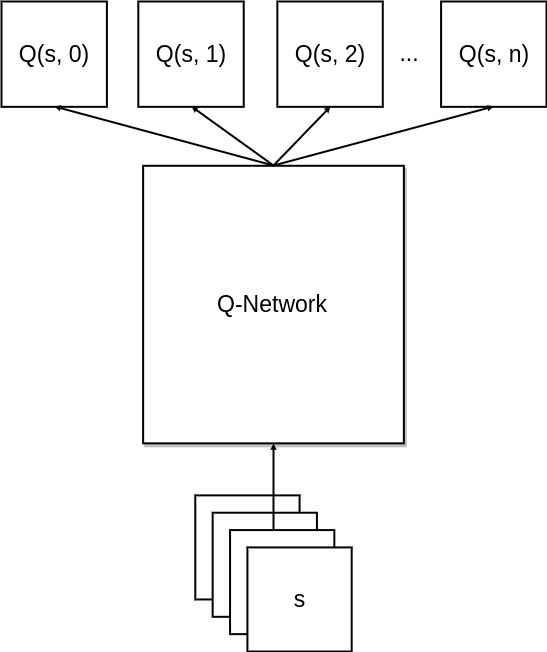
\includegraphics[width=0.4\textwidth]{pictures/dqn}
\centering
\caption{structure of the deep Q-network used by Mnih et al.\ in 
	 \cite{mnih2015human}. The network is trained to approximate the 
	 action-value function from the raw images of a game (used as states).}
\end{figure}
%
The key idea of deep Q-learning is to embed the update step of Q-learning into
the loss used for gradient descent to train a neural network (called 
\textit{deep Q-network}), resulting in the following gradient update:
%
\begin{IEEEeqnarray}{rCl}
    %
    \frac{\partial L}{\partial W_i^{old}} = E[(r + \gamma \max_{a'} Q(s', a') - Q(s, a)) \frac{\partial Q(s, a)}{\partial W_i^{old}}]
    %
\end{IEEEeqnarray}
%
The algorithm for deep Q-learning was introduced by Mnih et al. in \cite{mnih2015human}, using a
convolutional neural network with multidimensional output (one output neuron for
each action) as $Q$, and a set of samples collected with an exploratory policy 
from which the transitions for the update steps were sampled (a technique 
called \textit{experience replay}).
The CNN was structured to take as input a sequence of four frames (the states) 
from the games in the Atari suite of environments, and output an estimate of 
the action-value function which was then used to control the agent.
The samples used to update the estimates were collected with an $\varepsilon$-greedy
policy with a decaying $\varepsilon$ (hence the algorithm is \textit{off-policy}).
The algorithm proposed in the original paper is reported in Algorithm 
\ref{alg:DQL}.
%
\begin{algorithm}[h]
\caption{Deep Q-Learning with Experience Replay}
\label{alg:DQL}
    \begin{algorithmic}
	\STATE Initialize replay memory $\mathcal{D}$ to capacity $N$
	\STATE Initialize action-value function $Q$ with random weights
	\FOR{$episode = 1,M$}
	    \FOR{$t = 1,T$}
		\STATE Select a random action $a_t$ with probability $\varepsilon$
		\STATE Otherwise, select $a_t = \max_aQ^*(s_t, a)$
		\STATE Execute action $a_t$, collect reward $r_{t+1}$ and observe next state $s_{t+1}$
		\STATE Store the transition $(s_t, a_t, r_{t+1}, s_{t+1})$ in $\mathcal{D}$
		\STATE Sample random minibatch of transitions $(s_j, a_j, r_{j+1}, s_{j+1})$ from $\mathcal{D}$
		\STATE Set $ y_j = \begin{cases} r_j, & \mbox{if } s_{t+1}\mbox{ is terminal} \\ r_j + \max_{a'}Q(s_{t+1}, a'), & \mbox{otherwise}\end{cases}$
		\STATE Perform a gradient descent step using targets $y_j$
	    \ENDFOR
	\ENDFOR
    \end{algorithmic}
\end{algorithm}
%


